\documentclass[a4paper,12pt]{article}

\usepackage{latex_preamble/lab_preamble}

\begin{document}

% \Title{2.2.3}{Определение теплопроводности газов при атмосферном давлении}

\begin{titlepage}
  \begin{center}
    {\large МОСКОВСКИЙ ФИЗИКО-ТЕХНИЧЕСКИЙ ИНСТИТУТ (НАЦИОНАЛЬНЫЙ ИССЛЕДОВАТЕЛЬСКИЙ УНИВЕРСИТЕТ)}
  \end{center}
  \begin{center}
    {\large Физтех-школа прикладной математики и информатики}
  \end{center}

  \vspace{4.5cm}
  {\large
    \begin{center}
      {\bf Отчёт о выполнении лабораторной работы 2.2.3}\\
      Определение теплопроводности газов при атмосферном давлении
    \end{center}
  }
  \vspace{2cm}
  \begin{flushright}
    {\large Автор:\\ Чикин Андрей и Симонов Евгений\\
      \vspace{0.2cm}
      Б05-304}
  \end{flushright}
  \vspace{8cm}
  \begin{center}
    Долгопрудный, 2023
  \end{center}
\end{titlepage}

\tableofcontents
\listoffigures
\listoftables

\newpage

\textbf{Цель работы}:
\begin{enumerate}
  \item Определение коэффициента теплопроводности воздуха или углекислого газа при атмосферном давлении и разных температурах по теплоотдаче нагреваемой током нити в цилиндрическом сосуде
\end{enumerate}

\textbf{Приборы}:
\begin{enumerate}
  \item прибор для определения теплопроводности газов
  \item форвакуумный насос
  \item газгольдер с углекислым газом
  \item манометр
  \item магазин сопротивлений
  \item эталонное сопротивление 10 Ом
  \item цифровой вольтметр В7 --- 38
  \item источник питания
\end{enumerate}

\section{Краткая Теория.}
\quad{\it Теплопроводность} --- процесс, приводящий к выравниванию температуры в сосуде, где температура залючённого газа зависит от координат. Теплопроводность связана с тепловым движением молекул и не сопровождается макроскопическими перемещениями газа. \par
{\it Коэффициент теплопроводности} --- основная характеристика теплопроводности --- это коэффициент пропорциональности между плотностью потока тепла $q$ и градиентом температуры $dT/dr$ в направлении этого потока:

\begin{equation}
  q = -\kappa \frac{dT}{dr}
\end{equation} \par

В цилиндрически симметричной установке, в которой тепловой поток направлен к стенкам цилиндра от нити, полный поток тепла $Q = qS$ через каждую цилиндрическую поверхность радиуса $r$ должен в стационарном состоянии быть неизменен в пространстве и во времени. Тогда
\begin{equation}
  Q = -2\pi r L \kappa \frac{dT}{dr} = const
\end{equation}
\begin{description}
  \item[r] --- радиус цилиндра
  \item[L] --- высота цилиндра
\end{description}

откуда получаем:
\begin{equation}
  T_1 - T_2 = \frac{Q}{2\pi L \kappa} \ln{\frac{r2}{r1}}
\end{equation}\par
\begin{description}
  \item[$r_1$] --- радиус проволоки
  \item[$r_2$] --- радиус трубы с воздухом
\end{description}

В нашем эксперименте необходимо найти:
\begin{equation}
  \kappa = \frac{Q}{T_1-T_2}\frac{1}{2\pi L}\ln\frac{r2}{r1}
\end{equation}

\begin{equation}
  R(t)=R_{273}\cdot(1+\alpha t)
\end{equation}
\begin{equation}
  \alpha=\frac{1}{R_{273}}\frac{dR}{dT}
\end{equation}

$\alpha$ --- температурный коэффициент сопротивления материала.

\section{Экспериментальная установка}
Схема лабораторной установке представлена на рисунке \ref{fig:setup}. Тонкая молибденовая проволока натянута по оси вертикально стоящей медной трубки. Через штуцер трубка заполняется исследуемым газом. Нить нагревается электрическим током, ее температура $T_1$ определяется по изменению электрического сопротивления. Трубка находится в кожухе, через который пропускается вода из термостата. Температура воды $T_2$ измеряется термометром, помещенным в термостат. Количество теплоты,
протекающей через газ, равно (если пренебречь утечками тепла через торцы) количеству теплоты, выделяемому током в нити, и может быть найдено по закону Джоуля—Ленца. При этом ток в нити определяется по напряжению на включенном последовательно с ней эталонном сопротивлении 10 Ом. Таким образом, все величины, входящие в правую часть формулы (1), поддаются непосредственному измерению. \par
Электрическая часть схемы состоит из источника питания и под-
ключенных к нему последовательно соединенных нити, эталонного
сопротивления 10 Ом и магазина сопротивлений $R_M$, служащего для
точной установки тока через нить. Цифровой вольтметр может под-
ключаться как к нити, так и к эталонному сопротивлению, измеряя
таким образом напряжение на нити и ток через нее.

\begin{figure}[H]
  \centering
  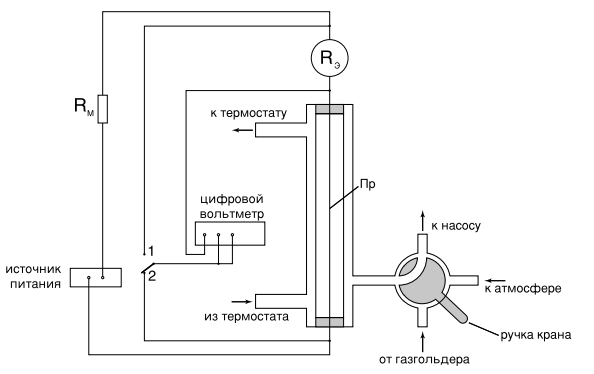
\includegraphics[width=0.7\textwidth]{data/setup.png}
  \caption{Схема установки для определения теплопроводности газов\label{fig:setup}}
\end{figure}

\begin{figure}[H]
  \centering
  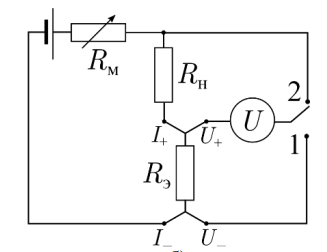
\includegraphics[width=0.3\textwidth]{data/circuit_fig.png}
  \caption{Электрическая схема установки.} \label{fig:circuit}
\end{figure}

\begin{description}
  \item[н] --- нить
  \item[э] --- эталон
\end{description}

\section{Обработка результатов измерений:}

\begin{table}[H]
  \begin{center}
    \begin{tabular}{|c|c|c|c|}
      \hline
      $L, \text{мм}$ & $2r_1, \text{мм}$ & $2r_2, \text{мм}$ & $R_{\text{э}}, \text{Ом}$
      \\\hline $367$ & $0.05$ & $10$ & $10$ \\\hline
    \end{tabular}
  \end{center}
  \caption{Параметры установки.\label{table:setup_pars}}
\end{table}

Для каждого измерения найдем ток, мощность, выделяемую в нити и сопротивление нити по формулам:

Закон Ома:
\begin{equation}
  I = \frac{U_{\text{э}}}{R_\text{э}}
\end{equation}

\begin{equation}
  Q = I U_{\text{н}} = U_{\text{н}} \frac{U_{\text{э}}}{R_{\text{э}}}
\end{equation}

\begin{equation}
  R_\text{н} = \frac{U_\text{н}}{I} =R_\text{э} \frac{U_\text{н}}{U_\text{э}}
\end{equation}


\begin{tabular}{|c|c|c|c|c|c|}
  \hline $T, K$ & $U_\text{э}, \text{мВ}$ & $U_{\text{н}}, \text{мВ}$ & $I, \text{мА}$ & $Q, \text{мВт}$ & $R_{\text{н}}, \text{Ом}$ \\\hline
  \multirow{8}{*}{297.5}
                & $ $                     & $1803.3$                  & $11.95$        & $12.96$         & $150.9$                   \\\cline{2-6}
                & $129.1$                 & $1949.7$                  & $12.91$        & $25.17$         & $151.0$                   \\\cline{2-6}
                & $170.1$                 & $2571.3$                  & $17.01$        & $43.72$         & $151.2$                   \\\cline{2-6}
                & $200.0$                 & $3028.2$                  & $20.00$        & $60.56$         & $151.4$                   \\\cline{2-6}
                & $224.5$                 & $3403.4$                  & $22.45$        & $76.41$         & $151.6$                   \\\cline{2-6}
                & $246.4$                 & $3740.3$                  & $24.64$        & $92.16$         & $151.8$                   \\\cline{2-6}
                & $264.9$                 & $4025.9$                  & $26.49$        & $106.67$        & $151.9$                   \\\cline{2-6}
                & $283.5$                 & $4312.3$                  & $28.35$        & $122.25$        & $152.1$                   \\\hline
  \multirow{8}{*}{308}
                & $100.1$                 & $1525.4$                  & $10.01$        & $15.27$         & $152.3$                   \\\cline{2-6}
                & $139.1$                 & $2121.4$                  & $13.91$        & $29.51$         & $152.4$                   \\\cline{2-6}
                & $170.8$                 & $2608.3$                  & $17.08$        & $44.56$         & $152.6$                   \\\cline{2-6}
                & $204.3$                 & $3095.7$                  & $20.43$        & $64.31$         & $152.8$                   \\\cline{2-6}
                & $221.3$                 & $3385.8$                  & $22.13$        & $74.92$         & $152.9$                   \\\cline{2-6}
                & $241.1$                 & $3692.7$                  & $24.11$        & $89.04$         & $153.1$                   \\\cline{2-6}
                & $260.5$                 & $3994.1$                  & $26.05$        & $104.04$        & $153.3$                   \\\cline{2-6}
                & $275.7$                 & $4230.3$                  & $27.57$        & $116.62$        & $153.4$                   \\\hline
  \multirow{8}{*}{318}
                & $98.0$                  & $1506.5$                  & $9.80$         & $14.77$         & $153.7$                   \\\cline{2-6}
                & $140.9$                 & $2169.2$                  & $14.9$         & $30.58$         & $153.9$                   \\\cline{2-6}
                & $170.9$                 & $2632.4$                  & $17.09$        & $44.98$         & $154.0$                   \\\cline{2-6}
                & $190.7$                 & $2940.0$                  & $19.07$        & $56.07$         & $154.1$                   \\\cline{2-6}
                & $220.5$                 & $3403.0$                  & $22.05$        & $75.01$         & $154.3$                   \\\cline{2-6}
                & $240.1$                 & $3710.1$                  & $24.01$        & $89.09$         & $154.5$                   \\\cline{2-6}
                & $260.2$                 & $4024.6$                  & $26.02$        & $104.72$        & $154.7$                   \\\cline{2-6}
                & $275.2$                 & $4260.8$                  & $27.52$        & $117.28$        & $154.8$                   \\\hline
  \multirow{8}{*}{328}
                & $98.1$                  & $1521.1$                  & $9.81$         & $14.92$         & $155.1$                   \\\cline{2-6}
                & $139.2$                 & $2160.4$                  & $13.92$        & $30.07$         & $155.2$                   \\\cline{2-6}
                & $170.0$                 & $2642.4$                  & $17.00$        & $44.93$         & $155.4$                   \\\cline{2-6}
                & $196.1$                 & $3050.6$                  & $19.61$        & $59.83$         & $155.5$                   \\\cline{2-6}
                & $219.0$                 & $3410.6$                  & $21.90$        & $74.69$         & $155.7$                   \\\cline{2-6}
                & $240.6$                 & $3749.9$                  & $24.06$        & $90.22$         & $155.8$                   \\\cline{2-6}
                & $259.1$                 & $4042.0$                  & $25.91$        & $104.72$        & $156.0$                   \\\cline{2-6}
                & $274.9$                 & $4292.7$                  & $27.49$        & $118.01$        & $156.1$                   \\\hline
  \multirow{8}{*}{338}
                & $98.0$                  & $1533.9$                  & $9.80$         & $15.04$         & $156.4$                   \\\cline{2-6}
                & $139.2$                 & $2160.4$                  & $13.92$        & $30.07$         & $156.5$                   \\\cline{2-6}
                & $169.2$                 & $2652.3$                  & $16.92$        & $44.87$         & $156.7$                   \\\cline{2-6}
                & $195.0$                 & $3059.6$                  & $19.50$        & $59.66$         & $156.9$                   \\\cline{2-6}
                & $218.2$                 & $3427.1$                  & $21.82$        & $74.78$         & $157.0$                   \\\cline{2-6}
                & $239.6$                 & $3767.1$                  & $23.96$        & $90.27$         & $157.2$                   \\\cline{2-6}
                & $258.8$                 & $4073.4$                  & $25.88$        & $105.39$        & $157.3$                   \\\cline{2-6}
                & $278.7$                 & $4309.7$                  & $27.87$        & $117.94$        & $157.5$                   \\\hline
\end{tabular} \\\\\\

Построим график зависимости сопротивления нити от температуры и из наклона графика найдём $dR/dT$:

Как видно, точки хорошо ложатся на прямую.
\[
  \frac{dR}{dT} = 0.13468
\]
Посчитаем температурный коэффициент сопротивления материала нити:
\[
  \alpha = \frac{1}{R_{273}} \frac{dR}{dT} = 0.9 \cdot 10^{-3} K^{-1}
\]
Построим для каждого $T$ графики зависимости $Q$ от $R$ и из наклонов графиков найдём $dQ/dT$:

\begin{tabular}{|c|c|c|c|c|c|}
  \hline
  $T, K$                                  & $297.5$         & $308$           & $318$           & $328$           & $338$           \\\hline
  $\frac{dQ_1}{dT},\ \frac{\text{Дж}}{K}$ & $0.0120$        & $0.0125$        & $0.0129$        & $0.0134$        & $0.0140$        \\\hline
  $\varkappa, \frac{\text{Вт}}{\text{м}}$ & $25.98 \pm 0.9$ & $26.62 \pm 1.0$ & $27.74 \pm 1.1$ & $28.55 \pm 1.1$ & $29.84 \pm 1.2$ \\\hline
  \\
\end{tabular}
Построим график $\ln\varkappa$ от $\ln T$:
% \begin{figure}[H]
%   \centering
%   \caption{Зависимость $\ln\varkappa$ от $\ln T$}
%   \includegraphics[scale=0.25]{zxc.png}
% \end{figure}
\[
  \frac{d\left(\ln \varkappa\right)}{d\left(\ln T\right)} = 1.08
\]
\section{Вывод:}
Я исследовал зависимость коэффицента теплопроводности от температуры, зависимость экспоненциальная, т.е. $\ln\varkappa$ от $\ln T$ зависит линейно, с коэффицентом наклона 1.08

\end{document}
